\documentclass{article}\usepackage[]{graphicx}\usepackage[]{xcolor}
% maxwidth is the original width if it is less than linewidth
% otherwise use linewidth (to make sure the graphics do not exceed the margin)
\makeatletter
\def\maxwidth{ %
  \ifdim\Gin@nat@width>\linewidth
    \linewidth
  \else
    \Gin@nat@width
  \fi
}
\makeatother

\definecolor{fgcolor}{rgb}{0.345, 0.345, 0.345}
\newcommand{\hlnum}[1]{\textcolor[rgb]{0.686,0.059,0.569}{#1}}%
\newcommand{\hlstr}[1]{\textcolor[rgb]{0.192,0.494,0.8}{#1}}%
\newcommand{\hlcom}[1]{\textcolor[rgb]{0.678,0.584,0.686}{\textit{#1}}}%
\newcommand{\hlopt}[1]{\textcolor[rgb]{0,0,0}{#1}}%
\newcommand{\hlstd}[1]{\textcolor[rgb]{0.345,0.345,0.345}{#1}}%
\newcommand{\hlkwa}[1]{\textcolor[rgb]{0.161,0.373,0.58}{\textbf{#1}}}%
\newcommand{\hlkwb}[1]{\textcolor[rgb]{0.69,0.353,0.396}{#1}}%
\newcommand{\hlkwc}[1]{\textcolor[rgb]{0.333,0.667,0.333}{#1}}%
\newcommand{\hlkwd}[1]{\textcolor[rgb]{0.737,0.353,0.396}{\textbf{#1}}}%
\let\hlipl\hlkwb

\usepackage{framed}
\makeatletter
\newenvironment{kframe}{%
 \def\at@end@of@kframe{}%
 \ifinner\ifhmode%
  \def\at@end@of@kframe{\end{minipage}}%
  \begin{minipage}{\columnwidth}%
 \fi\fi%
 \def\FrameCommand##1{\hskip\@totalleftmargin \hskip-\fboxsep
 \colorbox{shadecolor}{##1}\hskip-\fboxsep
     % There is no \\@totalrightmargin, so:
     \hskip-\linewidth \hskip-\@totalleftmargin \hskip\columnwidth}%
 \MakeFramed {\advance\hsize-\width
   \@totalleftmargin\z@ \linewidth\hsize
   \@setminipage}}%
 {\par\unskip\endMakeFramed%
 \at@end@of@kframe}
\makeatother

\definecolor{shadecolor}{rgb}{.97, .97, .97}
\definecolor{messagecolor}{rgb}{0, 0, 0}
\definecolor{warningcolor}{rgb}{1, 0, 1}
\definecolor{errorcolor}{rgb}{1, 0, 0}
\newenvironment{knitrout}{}{} % an empty environment to be redefined in TeX

\usepackage{alltt}

\title{Obtaining and Cleaning NOAA Weather Station Data}
\author{Marc Los Huertos}
\date{\today~(ver. 0.75)}
\IfFileExists{upquote.sty}{\usepackage{upquote}}{}
\begin{document}
\maketitle

\section{Introduction}

\subsection{Goals}

Using a list of active weather stations in the United States, you  will download and process the data to create a time series of temperature anomalies. 

\subsection{Read Data}

First, we install some packages and read in the data. I suggest you create a folder for the project (I created one called "04\_Regional\_Climate\_Trends") and then used the function here() to get the working directory and read the csv into R. This might be easier than the file.choose() option, but you can use that if you prefer.

\begin{knitrout}
\definecolor{shadecolor}{rgb}{0.969, 0.969, 0.969}\color{fgcolor}\begin{kframe}
\begin{alltt}
\hlkwd{library}\hlstd{(here)}
\end{alltt}


{\ttfamily\noindent\itshape\color{messagecolor}{\#\# here() starts at /home/mwl04747/RTricks}}\begin{alltt}
\hlkwd{library}\hlstd{(xtable)}

\hlstd{stations.active.oldest} \hlkwb{=} \hlkwd{read.csv}\hlstd{(}
  \hlkwd{here}\hlstd{(}\hlstr{"04_Regional_Climate_Trends"}\hlstd{,} \hlstr{"stations.active.oldest.csv"}\hlstd{))}

\hlcom{# OR}
\hlcom{# use file.choose() to select the file}
\hlcom{# filename = "MY.PATH/04_Regional_Climate_Trends/stations.active.oldest.csv"}
\hlcom{# stations.active.oldest = read.csv(filename)}
\end{alltt}
\end{kframe}
\end{knitrout}


\subsection{Map US Weather Stations}

Here's a map of the weather stations in the dataset. Pretty lame map!  We'll make a better one later.\footnote{Evelyn/Brody: This is a good change to see how to use R for map making! First we need to transform that data.}

\begin{knitrout}
\definecolor{shadecolor}{rgb}{0.969, 0.969, 0.969}\color{fgcolor}\begin{kframe}
\begin{alltt}
\hlkwd{plot}\hlstd{(stations.active.oldest}\hlopt{$}\hlstd{LONGITUDE,}
     \hlstd{stations.active.oldest}\hlopt{$}\hlstd{LATITUDE,}
     \hlkwc{xlab} \hlstd{=} \hlstr{"Longitude"}\hlstd{,}\hlkwc{ylab} \hlstd{=} \hlstr{"Latitude"}\hlstd{,}
     \hlkwc{pch}\hlstd{=}\hlnum{20}\hlstd{,} \hlkwc{cex}\hlstd{=}\hlnum{0.3}\hlstd{,} \hlkwc{col}\hlstd{=}\hlstr{'gray60'}\hlstd{,} \hlkwc{las}\hlstd{=}\hlnum{1}\hlstd{,}
     \hlkwc{main} \hlstd{=} \hlstr{"US Weather Stations"}\hlstd{)}
\end{alltt}
\end{kframe}
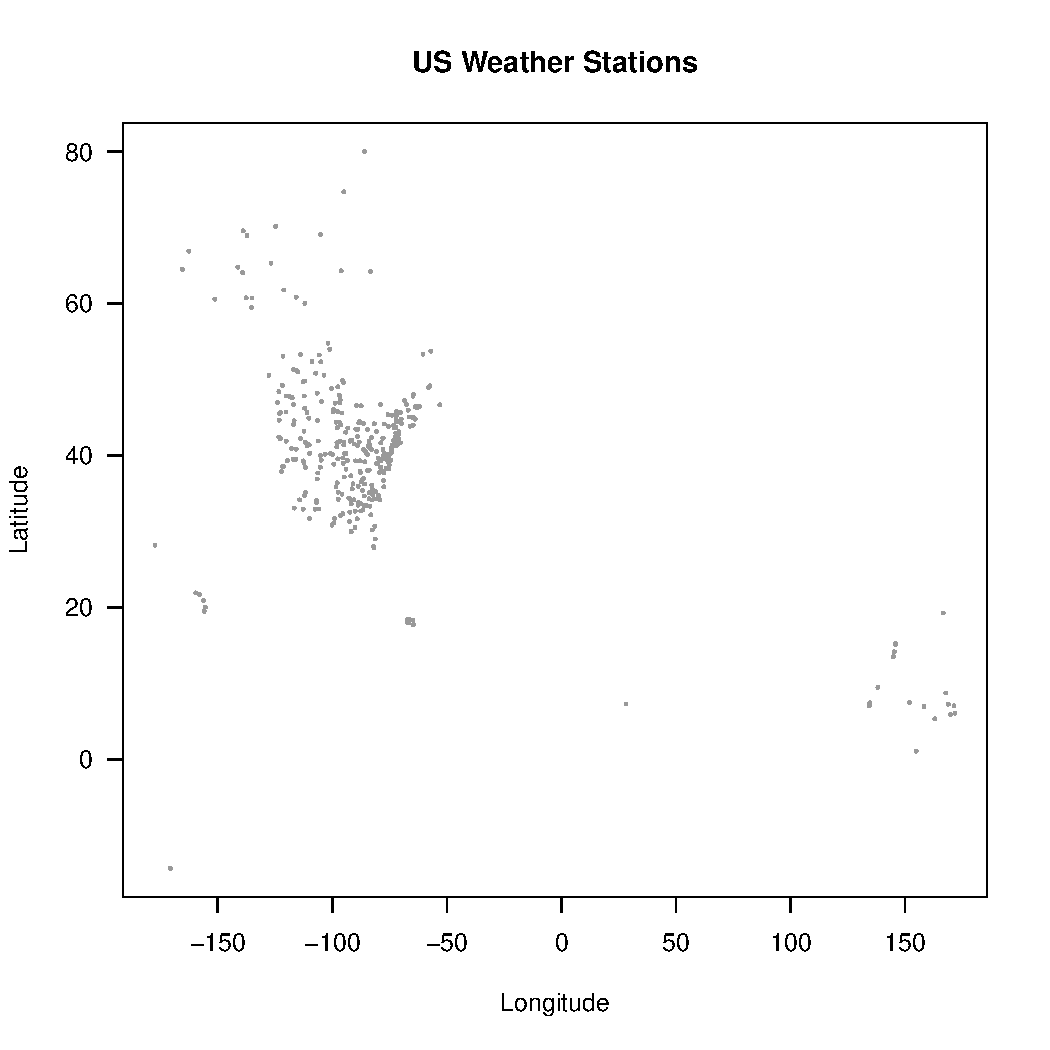
\includegraphics[width=\maxwidth]{figure/unnamed-chunk-2-1} 
\end{knitrout}
\subsection{Select and Evaluate State Data}

\begin{knitrout}
\definecolor{shadecolor}{rgb}{0.969, 0.969, 0.969}\color{fgcolor}\begin{kframe}
\begin{alltt}
\hlstd{stations.unique} \hlkwb{=}
  \hlkwd{unique}\hlstd{(stations.active.oldest[,}\hlkwd{c}\hlstd{(}\hlstr{"STATE"}\hlstd{,} \hlstr{"STATE_NAME"}\hlstd{)])}

\hlstd{xtab} \hlkwb{=} \hlkwd{xtable}\hlstd{(stations.unique)}
\end{alltt}
\end{kframe}
\end{knitrout}

The each of you will select a state -- see the Google Sheet sign up so we have a diverse set of states.

\begin{knitrout}
\definecolor{shadecolor}{rgb}{0.969, 0.969, 0.969}\color{fgcolor}\begin{kframe}
\begin{alltt}
\hlstd{my.state} \hlkwb{=} \hlstr{"CA"} \hlcom{# change the "CA" to your state}
\end{alltt}
\end{kframe}
\end{knitrout}

\section{Download Data from NOAA}

\subsection{Subset Station Data by State}

This uses the stations.active.oldest file to download the data from the NOAA website based on the state you have choose.

\begin{knitrout}
\definecolor{shadecolor}{rgb}{0.969, 0.969, 0.969}\color{fgcolor}\begin{kframe}
\begin{alltt}
\hlstd{my.stations} \hlkwb{=} \hlkwd{subset}\hlstd{(stations.active.oldest, STATE} \hlopt{==} \hlstd{my.state)}

\hlcom{# Download Updated Station Data}
\hlstd{i}\hlkwb{=}\hlnum{1}
\hlstd{here}\hlopt{::}\hlkwd{here}\hlstd{(}\hlstr{"04_Regional_Climate_Trends"}\hlstd{, my.stations}\hlopt{$}\hlstd{ID[i])}
\end{alltt}
\begin{verbatim}
## [1] "/home/mwl04747/RTricks/04_Regional_Climate_Trends/USC00043157"
\end{verbatim}
\end{kframe}
\end{knitrout}


The loop is not ideal -- loops are slow in R and prone to break -- but it should work for our purposes.\footnote{Evelyn/Brody: I wonder if we can test if the file exists so we don't have to downwload every time!} 
\begin{knitrout}
\definecolor{shadecolor}{rgb}{0.969, 0.969, 0.969}\color{fgcolor}\begin{kframe}
\begin{alltt}
\hlkwa{for}\hlstd{(i} \hlkwa{in} \hlnum{1}\hlopt{:}\hlkwd{nrow}\hlstd{(my.stations))\{}
  \hlstd{url} \hlkwb{=} \hlkwd{paste0}\hlstd{(}\hlstr{"https://www.ncei.noaa.gov/pub/data/ghcn/daily/by_station/"}\hlstd{,}
               \hlstd{my.stations}\hlopt{$}\hlstd{ID[i],}
               \hlstr{".csv.gz"}\hlstd{)}

\hlkwd{print}\hlstd{(i)} \hlcom{# Print Index Number}
\hlkwd{download.file}\hlstd{(url,} \hlkwd{paste0}\hlstd{(here}\hlopt{::}\hlkwd{here}\hlstd{(}\hlstr{"04_Regional_Climate_Trends"}\hlstd{,}
                                     \hlstr{"Data"}\hlstd{,}
                                     \hlstr{"SP24/"}\hlstd{),}
                          \hlstd{my.stations}\hlopt{$}\hlstd{ID[i],}
                          \hlstr{".csv.gz"}\hlstd{),}
              \hlkwc{quiet} \hlstd{=} \hlnum{FALSE}\hlstd{,} \hlkwc{mode} \hlstd{=} \hlstr{"w"}\hlstd{,} \hlkwc{cacheOK} \hlstd{=} \hlnum{TRUE}\hlstd{)}

\hlkwd{assign}\hlstd{(}\hlkwd{paste0}\hlstd{(}\hlstr{"station"}\hlstd{, i),}
       \hlkwd{read.csv}\hlstd{(}\hlkwd{gzfile}\hlstd{(}\hlkwd{paste0}\hlstd{(here}\hlopt{::}\hlkwd{here}\hlstd{(}\hlstr{"04_Regional_Climate_Trends"}\hlstd{,}
            \hlstr{"Data"}\hlstd{,} \hlstr{"SP24/"}\hlstd{),my.stations}\hlopt{$}\hlstd{ID[i],} \hlstr{".csv.gz"}\hlstd{)),}
            \hlkwc{header}\hlstd{=}\hlnum{FALSE}\hlstd{))}

\hlcom{# can't get the header named in loop! Grrr...}
\hlcom{#names(paste0("station",i)) <- c("ID", "DATE", "ELEMENT", }
\hlcom{# "VALUE", "M-FLAG", "Q-FLAG", "S-FLAG", "OBS-TIME")}

\hlstd{\}} \hlcom{# LOOP END}
\end{alltt}
\begin{verbatim}
## [1] 1
## [1] 2
## [1] 3
## [1] 4
## [1] 5
\end{verbatim}
\begin{alltt}
\hlcom{# Fix Variable Names based on NOAA Documentation}
\hlkwd{names}\hlstd{(station1)} \hlkwb{<-} \hlkwd{c}\hlstd{(}\hlstr{"ID"}\hlstd{,} \hlstr{"DATE"}\hlstd{,} \hlstr{"ELEMENT"}\hlstd{,} \hlstr{"VALUE"}\hlstd{,}
                     \hlstr{"M-FLAG"}\hlstd{,} \hlstr{"Q-FLAG"}\hlstd{,} \hlstr{"S-FLAG"}\hlstd{,} \hlstr{"OBS-TIME"}\hlstd{)}
\hlkwd{names}\hlstd{(station3)} \hlkwb{<-} \hlkwd{names}\hlstd{(station2)} \hlkwb{<-} \hlkwd{names}\hlstd{(station1)}
\hlkwd{names}\hlstd{(station5)} \hlkwb{<-} \hlkwd{names}\hlstd{(station4)} \hlkwb{<-} \hlkwd{names}\hlstd{(station1)}

\hlcom{# NAMES OF VARIABLES ARE INCORRECT for some STATIONS??}

  \hlcom{#ID = 11 character station identification code}
  \hlcom{#YEAR/MONTH/DAY = 8 character date in YYYYMMDD format }
  \hlcom{#                     (e.g. 19860529 = May 29, 1986)}
  \hlcom{#ELEMENT = 4 character indicator of element type }
  \hlcom{#DATA VALUE = 5 character data value for ELEMENT }
  \hlcom{#M-FLAG = 1 character Measurement Flag }
  \hlcom{#Q-FLAG = 1 character Quality Flag }
  \hlcom{#S-FLAG = 1 character Source Flag }
  \hlcom{#OBS-TIME = 4-character time of observation in hour-minute format}
  \hlcom{#                     (i.e. 0700 =7:00 am); if no ob time information }
 \hlcom{#is available, the field is left empty}
\end{alltt}
\end{kframe}
\end{knitrout}

\section{Process and Clean Data}


I have created a "function" that can process and clean the data, if the data are consistent!  If not, we'll trouble shoot together. 

Here's the data structure, using str(), but if you have something different, please let me know and we'll sort out how to fix it. 

\begin{knitrout}
\definecolor{shadecolor}{rgb}{0.969, 0.969, 0.969}\color{fgcolor}\begin{kframe}
\begin{alltt}
\hlkwd{str}\hlstd{(station1)}
\end{alltt}
\begin{verbatim}
## 'data.frame':	224921 obs. of  8 variables:
##  $ ID      : chr  "USC00043157" "USC00043157" "USC00043157" "USC00043157" ...
##  $ DATE    : int  18670601 18670602 18670603 18670604 18670605 18670606 18670607 18670608 18670609 18670610 ...
##  $ ELEMENT : chr  "PRCP" "PRCP" "PRCP" "PRCP" ...
##  $ VALUE   : int  0 0 0 0 0 0 0 0 0 0 ...
##  $ M-FLAG  : chr  "" "" "" "" ...
##  $ Q-FLAG  : chr  "" "" "" "" ...
##  $ S-FLAG  : chr  "F" "F" "F" "F" ...
##  $ OBS-TIME: int  NA NA NA NA NA NA NA NA NA NA ...
\end{verbatim}
\end{kframe}
\end{knitrout}


\subsection{Clean Data}

First, I tested each line on station1. I will then create a function to clean the data and apply it to each station.

\begin{knitrout}
\definecolor{shadecolor}{rgb}{0.969, 0.969, 0.969}\color{fgcolor}\begin{kframe}
\begin{alltt}
\hlstd{station1}\hlopt{$}\hlstd{VALUE} \hlkwb{=} \hlstd{station1}\hlopt{$}\hlstd{VALUE}\hlopt{/}\hlnum{10}  \hlcom{# Correct Values Units}
\hlcom{# Fix Date format}
\hlstd{station1}\hlopt{$}\hlstd{Ymd} \hlkwb{=} \hlkwd{as.Date}\hlstd{(}\hlkwd{as.character}\hlstd{(station1}\hlopt{$}\hlstd{DATE),} \hlkwc{format} \hlstd{=} \hlstr{"%Y%m%d"}\hlstd{)}
\hlkwd{str}\hlstd{(station1)}
\end{alltt}
\begin{verbatim}
## 'data.frame':	224921 obs. of  9 variables:
##  $ ID      : chr  "USC00043157" "USC00043157" "USC00043157" "USC00043157" ...
##  $ DATE    : int  18670601 18670602 18670603 18670604 18670605 18670606 18670607 18670608 18670609 18670610 ...
##  $ ELEMENT : chr  "PRCP" "PRCP" "PRCP" "PRCP" ...
##  $ VALUE   : num  0 0 0 0 0 0 0 0 0 0 ...
##  $ M-FLAG  : chr  "" "" "" "" ...
##  $ Q-FLAG  : chr  "" "" "" "" ...
##  $ S-FLAG  : chr  "F" "F" "F" "F" ...
##  $ OBS-TIME: int  NA NA NA NA NA NA NA NA NA NA ...
##  $ Ymd     : Date, format: "1867-06-01" "1867-06-02" ...
\end{verbatim}
\begin{alltt}
\hlstd{station1}\hlopt{$}\hlstd{MONTH} \hlkwb{=} \hlkwd{as.numeric}\hlstd{(}\hlkwd{format}\hlstd{(station1}\hlopt{$}\hlstd{Ymd,} \hlstr{"%m"}\hlstd{))}
\hlstd{station1}\hlopt{$}\hlstd{YEAR} \hlkwb{=} \hlkwd{as.numeric}\hlstd{(}\hlkwd{format}\hlstd{(station1}\hlopt{$}\hlstd{Ymd,} \hlstr{"%Y"}\hlstd{))}
\hlstd{station1.monthly} \hlkwb{=} \hlkwd{aggregate}\hlstd{(VALUE} \hlopt{~} \hlstd{MONTH} \hlopt{+} \hlstd{YEAR,}
                   \hlkwc{data} \hlstd{=} \hlkwd{subset}\hlstd{(station1, ELEMENT} \hlopt{==} \hlstr{"TMAX"}\hlstd{), mean)}

\hlcom{# create baseline (normals) dataset}
\hlstd{station1.normals} \hlkwb{=} \hlkwd{subset}\hlstd{(station1,}
                           \hlstd{Ymd} \hlopt{>=} \hlstr{"1961-01-01"} \hlopt{&} \hlstd{Ymd} \hlopt{<=} \hlstr{"1990-12-31"}\hlstd{)}
\hlstd{station1.normals.monthly} \hlkwb{=} \hlkwd{aggregate}\hlstd{(VALUE} \hlopt{~} \hlstd{MONTH,}
                   \hlkwc{data} \hlstd{=} \hlkwd{subset}\hlstd{(station1.normals, ELEMENT} \hlopt{==} \hlstr{"TMAX"}\hlstd{), mean)}
\hlkwd{names}\hlstd{(station1.normals.monthly)} \hlkwb{<-} \hlkwd{c}\hlstd{(}\hlstr{"MONTH"}\hlstd{,} \hlstr{"NORMALS"}\hlstd{)}

\hlstd{station1.anomaly} \hlkwb{=} \hlkwd{merge}\hlstd{(station1.monthly,}
                         \hlstd{station1.normals.monthly,} \hlkwc{by} \hlstd{=} \hlstr{"MONTH"}\hlstd{)}
\hlstd{station1.anomaly}\hlopt{$}\hlstd{ANOMALY} \hlkwb{=}
  \hlstd{station1.anomaly}\hlopt{$}\hlstd{VALUE} \hlopt{-} \hlstd{station1.anomaly}\hlopt{$}\hlstd{NORMALS}
\end{alltt}
\end{kframe}
\end{knitrout}

\subsection{Clean Data Function}

Function is probably senstive to missing values, need to work on that!

\begin{knitrout}
\definecolor{shadecolor}{rgb}{0.969, 0.969, 0.969}\color{fgcolor}\begin{kframe}
\begin{alltt}
\hlstd{cleandataframe.fun} \hlkwb{<-} \hlkwa{function}\hlstd{(}\hlkwc{x}\hlstd{)\{}
  \hlstd{x}\hlopt{$}\hlstd{VALUE} \hlkwb{=} \hlstd{x}\hlopt{$}\hlstd{VALUE}\hlopt{/}\hlnum{10}
  \hlstd{x}\hlopt{$}\hlstd{Ymd} \hlkwb{=} \hlkwd{as.Date}\hlstd{(}\hlkwd{as.character}\hlstd{(x}\hlopt{$}\hlstd{DATE),} \hlkwc{format} \hlstd{=} \hlstr{"%Y%m%d"}\hlstd{)}
  \hlstd{x}\hlopt{$}\hlstd{MONTH} \hlkwb{=} \hlkwd{as.numeric}\hlstd{(}\hlkwd{format}\hlstd{(x}\hlopt{$}\hlstd{Ymd,} \hlstr{"%m"}\hlstd{))}
  \hlstd{x}\hlopt{$}\hlstd{YEAR} \hlkwb{=} \hlkwd{as.numeric}\hlstd{(}\hlkwd{format}\hlstd{(x}\hlopt{$}\hlstd{Ymd,} \hlstr{"%Y"}\hlstd{))}
  \hlstd{x.monthly} \hlkwb{=} \hlkwd{aggregate}\hlstd{(VALUE} \hlopt{~} \hlstd{MONTH} \hlopt{+} \hlstd{YEAR,}
                   \hlkwc{data} \hlstd{=} \hlkwd{subset}\hlstd{(x, ELEMENT} \hlopt{==} \hlstr{"TMAX"}\hlstd{), mean)}
  \hlstd{x.normals} \hlkwb{=} \hlkwd{subset}\hlstd{(x, Ymd} \hlopt{>=} \hlstr{"1961-01-01"} \hlopt{&} \hlstd{Ymd} \hlopt{<=} \hlstr{"1990-12-31"}\hlstd{)}
  \hlstd{x.normals.monthly} \hlkwb{=} \hlkwd{aggregate}\hlstd{(VALUE} \hlopt{~} \hlstd{MONTH,}
                   \hlkwc{data} \hlstd{=} \hlkwd{subset}\hlstd{(x.normals, ELEMENT} \hlopt{==} \hlstr{"TMAX"}\hlstd{), mean)}
  \hlkwd{names}\hlstd{(x.normals.monthly)} \hlkwb{<-} \hlkwd{c}\hlstd{(}\hlstr{"MONTH"}\hlstd{,} \hlstr{"NORMALS"}\hlstd{)}
  \hlstd{x.anomaly} \hlkwb{=} \hlkwd{merge}\hlstd{(x.monthly, x.normals.monthly,} \hlkwc{by} \hlstd{=} \hlstr{"MONTH"}\hlstd{)}
  \hlstd{x.anomaly}\hlopt{$}\hlstd{ANOMALY} \hlkwb{=} \hlstd{x.anomaly}\hlopt{$}\hlstd{VALUE} \hlopt{-} \hlstd{x.anomaly}\hlopt{$}\hlstd{NORMALS}
  \hlkwd{return}\hlstd{(x.anomaly)}
\hlstd{\}}
\end{alltt}
\end{kframe}
\end{knitrout}

\subsection{Apply Function to All Stations}

So far, I have only run function for 1 station, but I suspect you can figure out how to run it for each one!

\begin{knitrout}
\definecolor{shadecolor}{rgb}{0.969, 0.969, 0.969}\color{fgcolor}\begin{kframe}
\begin{alltt}
\hlstd{station1.TMAX} \hlkwb{=} \hlkwd{cleandataframe.fun}\hlstd{(station1)}
\end{alltt}
\end{kframe}
\end{knitrout}

\subsection{Plot Anomaly}

Graphic has lots of issues. more next time!  But here's a start.

\begin{knitrout}
\definecolor{shadecolor}{rgb}{0.969, 0.969, 0.969}\color{fgcolor}\begin{kframe}
\begin{alltt}
\hlkwd{options}\hlstd{(}\hlkwc{scipen}\hlstd{=}\hlnum{5}\hlstd{)}
\hlkwd{par}\hlstd{(}\hlkwc{mar}\hlstd{=}\hlkwd{c}\hlstd{(}\hlnum{4}\hlstd{,}\hlnum{6}\hlstd{,}\hlnum{2}\hlstd{,}\hlnum{5}\hlstd{))}

\hlkwd{plot}\hlstd{(ANOMALY} \hlopt{~} \hlstd{YEAR,} \hlkwc{data} \hlstd{=} \hlkwd{subset}\hlstd{(station1.TMAX, MONTH} \hlopt{==} \hlnum{1}\hlstd{),}
     \hlkwc{las}\hlstd{=}\hlnum{1}\hlstd{,} \hlkwc{pch}\hlstd{=}\hlnum{19}\hlstd{,} \hlkwc{col} \hlstd{=} \hlstr{"blue"}\hlstd{,} \hlkwc{cex}\hlstd{=}\hlnum{.5}\hlstd{,} \hlcom{#xlab = "Year", }
     \hlkwc{ylab} \hlstd{=} \hlstr{"Maximum Temp Anomaly (C)"}\hlstd{,}
     \hlkwc{main}\hlstd{=}\hlstr{"January Maximum Temp Anomaly"}\hlstd{)}
\hlkwd{mtext}\hlstd{(}\hlstr{"Maximum Temp Anomaly (C)"}\hlstd{,} \hlkwc{side} \hlstd{=} \hlnum{2}\hlstd{,} \hlkwc{line} \hlstd{=} \hlnum{3}\hlstd{)}
\hlstd{temp.lm} \hlkwb{=} \hlkwd{lm}\hlstd{(ANOMALY} \hlopt{~} \hlstd{YEAR,} \hlkwc{data} \hlstd{=} \hlkwd{subset}\hlstd{(station1.TMAX, MONTH} \hlopt{==} \hlnum{1}\hlstd{))}
\hlkwd{abline}\hlstd{(}\hlkwd{coef}\hlstd{(temp.lm),} \hlkwc{col} \hlstd{=} \hlstr{"red"}\hlstd{)}
\end{alltt}
\end{kframe}
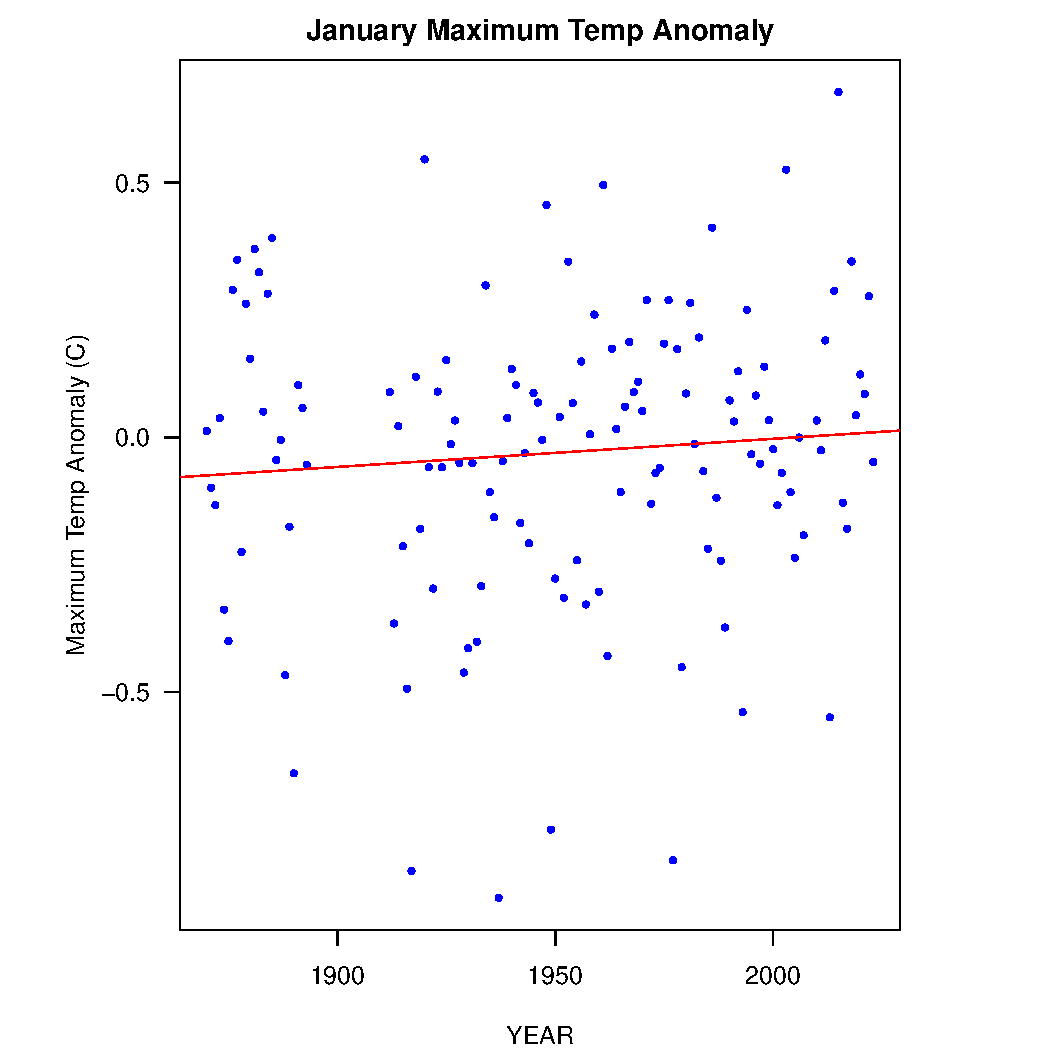
\includegraphics[width=\maxwidth]{figure/unnamed-chunk-10-1} 
\end{knitrout}


\section{Next Steps}

This is all we need to do so far. Next week, we'll look at different way to visualize the data!


write.csv(station1.TMAX, file = "station1.TMAX.csv", row.names = FALSE)
write.csv(station2.TMAX, file = "station2.TMAX.csv", row.names = FALSE)
write.csv(station3.TMAX, file = "station3.TMAX.csv", row.names = FALSE)
write.csv(station4.TMAX, file = "station4.TMAX.csv", row.names = FALSE)
write.csv(station5.TMAX, file = "station5.TMAX.csv", row.names = FALSE)


\end{document}
